\documentclass[red]{beamer}
\usepackage[utf8]{inputenc}
\usepackage[T1]{fontenc}

\usetheme{Ilmenau}
\usecolortheme{beaver}
\setbeamercolor{institute in head/foot}{fg=darkred}
\setbeamercolor{navigation symbols}{fg=darkred}
\setbeamertemplate{itemize item}[circle]
\setbeamertemplate{blocks}[rounded][shadow=false]
% Mieux sans, non ?
%\setbeamertemplate{sections/subsections in toc}[sections numbered]
\setbeamertemplate{navigation symbols}{\hspace{\stretch{1}}\insertframenumber/\inserttotalframenumber\hspace{\stretch{1}}}
\setbeamertemplate{blocks}[rounded][shadow=true]

%\AtBeginSection[]
%{
%    \begin{frame}
%        \frametitle{Plan}
%        {\small \tableofcontents}
%    \end{frame} 
%}

%\logo{
\includegraphics[height=0.15\textwidth]{img/logo.jpg}}

\title[RE315 : Laptop]{RE315 - Sécurité des Réseaux\\
                       \textsc{Projet Laptop}}
\author{J.\textsc{Chaumont} \and P.\textsc{Gourinchas}\\
        \and A.\textsc{Hanriat} \and F.\textsc{Monjalet}}
\institute{ENSEIRB-MATMECA}
\date{27 janvier 2014}

\begin{document}

{
\logo{}
\setbeamertemplate{navigation symbols}{}
\setbeamertemplate{headline}{}
\begin{frame}
    \vspace{-0.2cm}
    \maketitle
    \vspace{-0.7cm}
    \begin{center}
        
\includegraphics[height=0.29\textheight]{img/logo.jpg}

    \end{center}
\end{frame}
}

%%%%%%%%%%%%%%%%%%%%%%%%%%%Présentation
\addtocounter{framenumber}{-1}
\section{Introduction}
\begin{frame}
    \frametitle{Introduction}
    \begin{block}{Objectifs}
        \begin{itemize}
            \item Attaques non cryptographiques contre disques durs
            chiffrés
            \item Leaker le mot de passe ou la clé de chiffrement par
            un moyen de notre choix
            \item Supposition d'un accès physique/root à la machine
        \end{itemize}
    \end{block}
    \begin{block}{Enjeux}
        \begin{itemize}
            \item Forensic, affaires judiciaires
            % Exemple du gros bonnet Brézilien
            \item Protection des données
            % Est-ce vraiment possible ?
        \end{itemize}
    \end{block}
\end{frame}

%%%%%%%%%%%%%%%%%%%%%%%%%%%Plan
\begin{frame}
    \frametitle{Plan}
    \tableofcontents
\end{frame}

%%%%%%%%%%%%%%%%%%%%%%%%%%%LUKS
\section{LUKS}
\subsection{Présentation}
\begin{frame}
    \frametitle{LUKS}
    \begin{block}{Présentation}
        \begin{itemize}
            \item Norme de chiffrement de disques (2005)
            \item Proposée par les distributions GNU/Linux
            \item Différentes implémentations
        \end{itemize}
    \end{block}
    \centering
    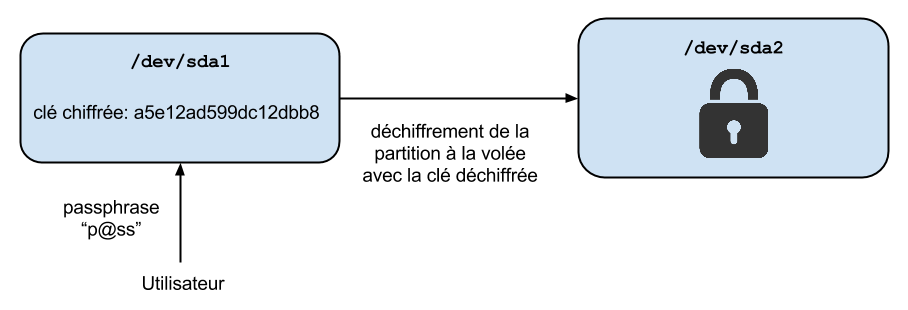
\includegraphics[width=10.8cm]{img/luks_principe.png}
\end{frame}


\begin{frame}
    \frametitle{Principe de l'attaque}
    \begin{block}{Pré-requis}
        \begin{itemize}
            \item Accès physique
            \begin{itemize}
                \item Hypothèse : attaque \textit{Evil Maid}
                \item Être root sur la machine via un live OS
            \end{itemize}
        \item Ou accès root sur un système déjà présent sur la 
        machine
        \end{itemize}
    \end{block}
    \pause
    
    \begin{block}{\'Etapes}
        \begin{enumerate}
            \item Infection de la partition en clair
            \item Interception du mot de passe utilisateur
            \item Récupération du mot de passe
        \end{enumerate}
    \end{block}
\end{frame}

\subsection{Réalisation}
\begin{frame}
    \frametitle{Sous Debian}
    \begin{block}{Principe}
        \begin{itemize}
            \item Compromission du \texttt{initrd}
            \begin{itemize}
                \item Insertion d'une backdoor dans \texttt{cryptroot}
            \end{itemize}
            \item Récupération temporaire du mot de passe saisi
            \item Accès en écriture au système chiffré une fois monté
            via compromission d'\texttt{init}
            \item Exploitation du \texttt{rc.local} et effacement des
            traces
        \end{itemize}
    \end{block}
\end{frame}


\begin{frame}
    \frametitle{Sous Fedora}
    \begin{block}{Principe}
        \begin{itemize}
            \item Compromission du \texttt{initramfs}
            \begin{itemize}
                \item Recompilation de \texttt{systemd-cryptsetup} dans \textit{systemd}
            \end{itemize}
            \item Récupération temporaire du mot de passe saisi
            \item Exploitation des secteurs inutilisés du \textit{ext4}
            \item Récupération du mot de passe par l'attaquant et effacement des traces
        \end{itemize}
    \end{block}

\end{frame}


\begin{frame}
    \frametitle{Démonstration}
    \centering
    Démonstration sous Fedora
    \vspace{0.5cm}
    
    
\includegraphics[width=2cm]{img/fedora_logo.png}
\end{frame}

%%%%%%%%%%%%%%%%%%%%%%%%%%%TrueCrypt
\section{TrueCrypt}
\subsection{Présentation}
\begin{frame}
    \frametitle{TrueCrypt}
    \begin{itemize}
        \item Outil de chiffrement très réputé (dit NSA proof)
        \item Sources fournies : facilite l'attaque
        \item Compilation "maison" non utilisable pour Windows, car
        le binaire doit être signé
        % Problématiques d'intégrité : le binaire correspond-il
        % aux sources ?
        \item Multi Plateforme (Windows, Linux, Mac OS X)
        \item Plusieurs possibilités de chiffrement :
        \begin{itemize}
            \item Chiffrement de dossiers
            \item Chiffrement de partitions
            \item \textbf{Chiffrement de disques complets}
        \end{itemize}
        \item Phishing
    \end{itemize}
\end{frame}

\begin{frame}
    \frametitle{Séquence de boot}
    \vspace{-0.6cm}
    \begin{center}
        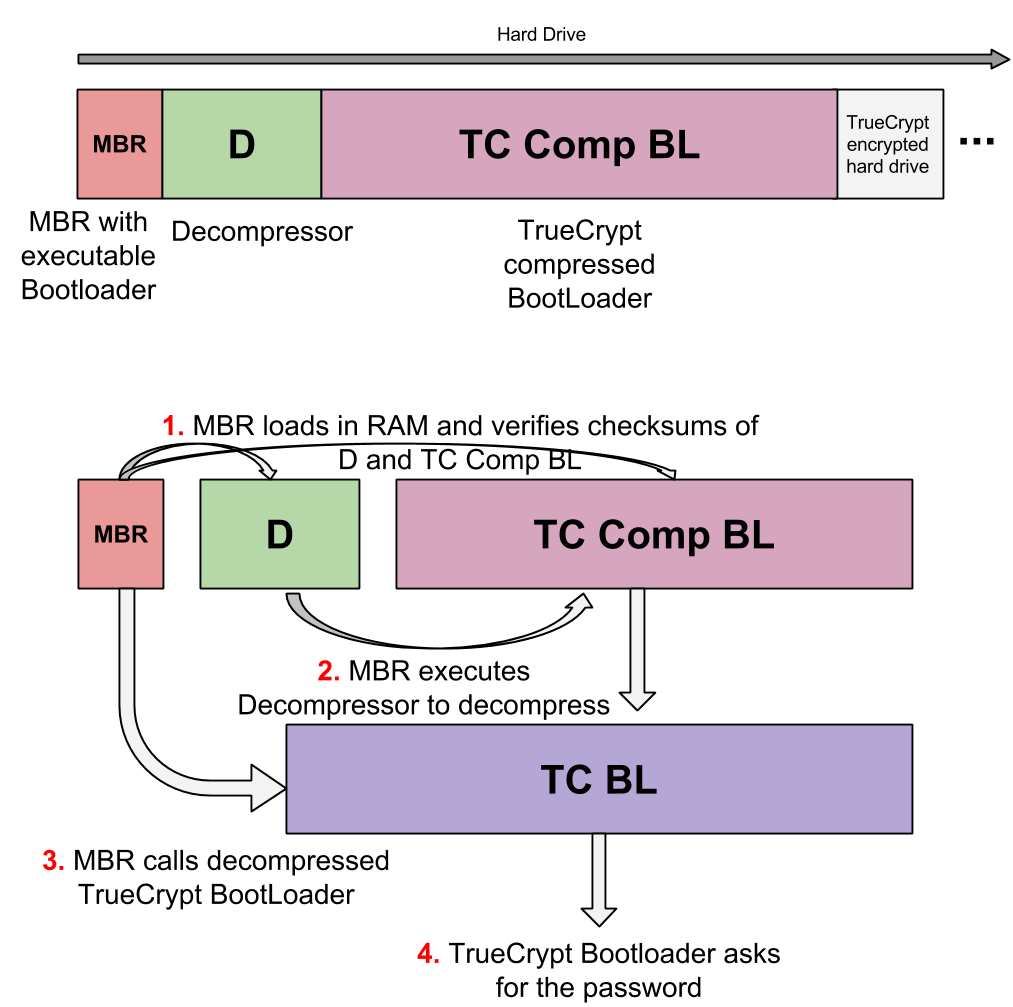
\includegraphics[height=0.85\textheight]{img/tc_boot.png}
    \end{center}
\end{frame}

\subsection{L'attaque}
\begin{frame}
    \frametitle{L'attaque}
    \begin{block}{Idée}
        \begin{itemize}
            \item \texttt{void AskPassword(Password \&password);}
            \item Corrompre le secteur de boot pour leaker le mot de
            passe
            \item Intercepter un appel en intercalant un appel à un
            code malicieux dumpant le mot de passe
        \end{itemize}
    \end{block}
\end{frame}

\begin{frame}
    \begin{center}
        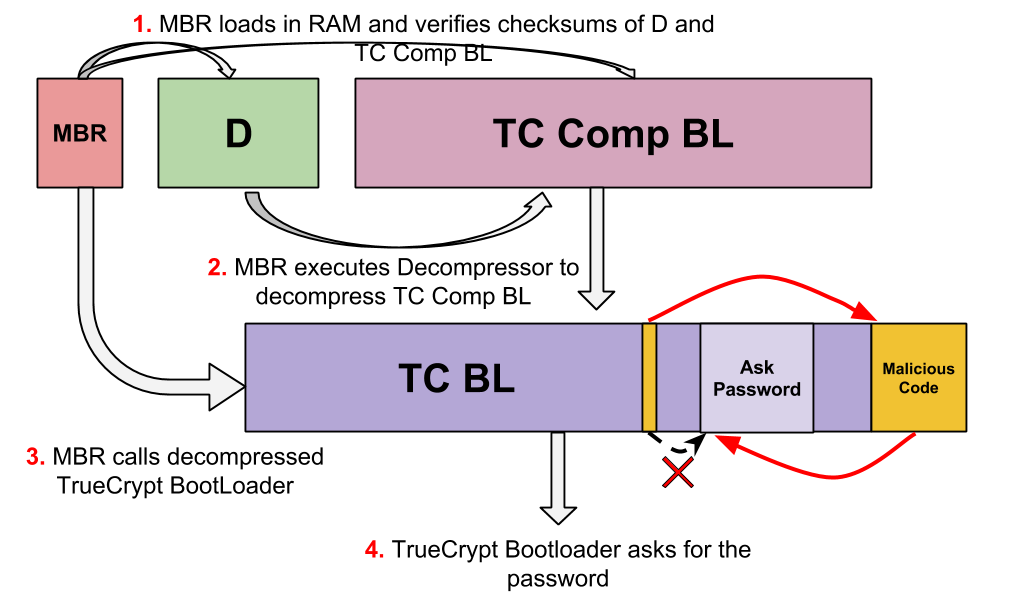
\includegraphics[width=0.9\textwidth]{img/tc_boot_min.png}
    \end{center}
\end{frame}

\begin{frame}
    \frametitle{Code malicieux}
    \begin{columns}
    \column{0.40\textwidth}
        Fonctionnement :
        \begin{enumerate}
            \item Réempiler l'adresse de l'argument de
            \texttt{AskPassword}
            \item Appeler \texttt{AskPassword}
            \item Écrire le contenu de l'argument une fois rempli
            sur un secteur libre du disque dur (via \texttt{int 0x13})
        \end{enumerate}
        
        Quel secteur libre ?
        
        Autre solution ? % Selon le temps
        
    \column{0.65\textwidth}
        \vspace{-1.5cm}
        \begin{center}
            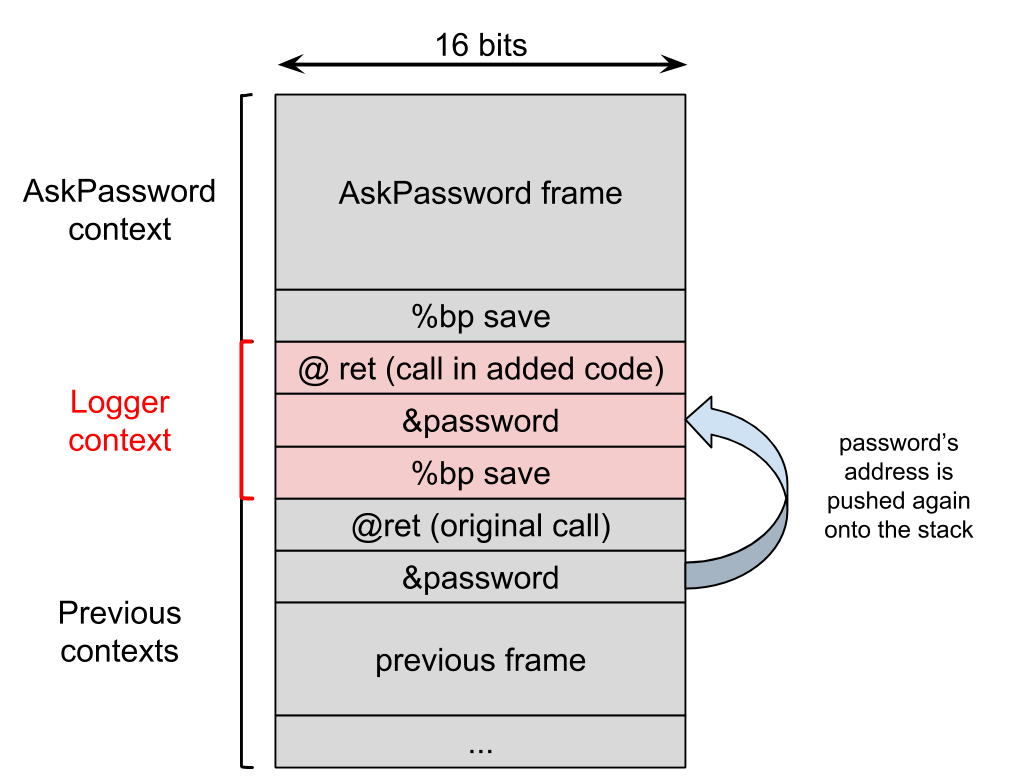
\includegraphics[height=0.65\textheight]{img/pile_tc.png}
        \end{center}
    \end{columns}
\end{frame}

\begin{frame}
    \frametitle{En résumé}
    Si la machine n'est \textbf{pas} déjà infectée :
    \begin{enumerate}
        \item Décompression du bootloader via GZip
        \item Ajout du code malicieux
        \item Changement des offsets des \textit{call}s pour appeler
        le code malicieux, et que celui-ci appelle \texttt{AskPassword}
        \item Recompresser et réécrire le bootloader patché
        \item Patcher le MBR (checksum, taille du bootloader)
    \end{enumerate}
    Si la machine est \textbf{déjà} infectée :
    \begin{itemize}
        \item Lire la structure \texttt{Password} dumpée
    \end{itemize}
    ~\\
    
    Possibilité théorique de remonter jusqu'à une infection système.
\end{frame}

\begin{frame}
    \frametitle{Démonstration}
    \begin{center}
        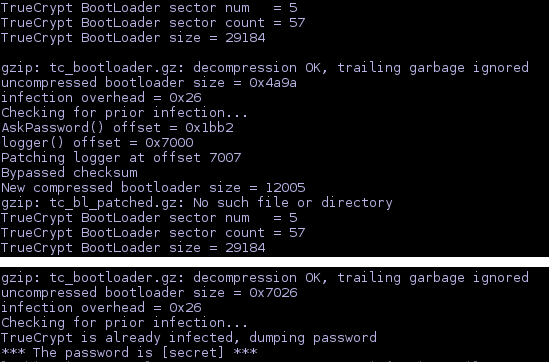
\includegraphics[height=0.8\textheight]{img/demo_tc.png}
    \end{center}
\end{frame}

%%%%%%%%%%%%%%%%%%%%%%%%%%%BitLocker
\section{BitLocker}
\subsection{Présentation}
\begin{frame}
    \frametitle{Présentation}
    Système de chiffrement de disque dur de Microsoft.
    \begin{block}{Trois modes de fonctionnement}
        \begin{itemize}
            \item Avec TPM
                \begin{itemize}
                    \item Sans authentification de l'utilisateur
                    \item Avec authentification de l'utilisateur
                \end{itemize}
            \item Sans TPM: utilisation d'une clé USB
        \end{itemize}
    \end{block}
    \begin{block}{TPM (Trusted Platform Module)}
        \begin{itemize}
            \item Composant matériel (plutôt cher)
            \item Se lance avant le BIOS
            \item Détection des modifications au démarrage
            \item Contient les clés de chiffrement
        \end{itemize}
    \end{block}
\end{frame}

\subsection{Idée d'attaque}
\begin{frame}
    \frametitle{Idée d'attaque}
    \begin{description}
        \item[Avec TPM] Compromission du TPM très complexe, mais réalisable.
        \item[Sans TPM] Fichier d'authentification stocké sur une clé USB. La copie du fichier donne l'accès au disque.
    \end{description}
\end{frame}

%%%%%%%%%%%%%%%%%%%%%%%%%%%RAM + USB
\section{Autres méthodes et vecteur d'attaque}
\subsection{Dump mémoire}
\begin{frame}
    \frametitle{Dump mémoire}
    \begin{center}
    {\LARGE Pourquoi dumper la mémoire ?} ~~\\
    \end{center}
    %% Les différentes méthodes de dump mémoire
    Les différentes manières de récupérer la mémoire physique
    \begin{itemize}
        \item Cold boot attack
        \item Via port Firewire
        \item Dump mémoire / récupération fichier hibernation  via OS bootable 
    \end{itemize}
    %% Présentation de celle qu'on a retenue (contraintes ect..
    \begin{block}{Solution retenue}
    Adaptation d'un mini OS (< 12MB) sur clé USB 
    \end{block}
\end{frame}

\subsection{Vecteur d'attaque et application}
\begin{frame}
    \frametitle{Recompilation du kernel}
    Depuis la version 2.6, on ne peut plus avoir accès à toute la mémoire virtuelle via \texttt{/dev/mem} \\
    Possiblité de recompiler le noyau avec les bonnes options :

    ~~ \\
    \centering
        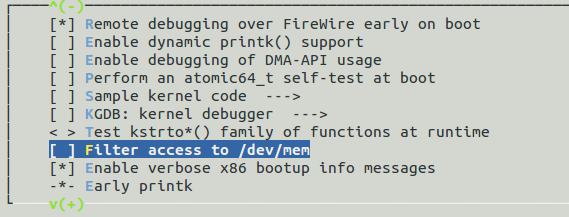
\includegraphics[height=0.40\textheight]{img/kernel.png}

    Accès uniquement à la mémoire virtuelle !
    %% Pourquoi recompiler le kernel ?
\end{frame}

\begin{frame}
    \frametitle{Insertion du module kernel fmem.ko}
    \begin{block}{fmem}
    \textbf{fmem} est un module noyau permettant d'avoir accès à \textbf{toute} la mémoire
    sans devoir recompiler le noyau.
    ~~ \\
    \centering
        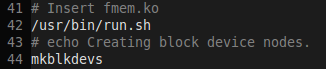
\includegraphics[height=0.2\textheight]{img/init.png}
    \end{block}
    %% Qu'est ce que fmem.ko ?
    %% Explication de l'insertion du module dans init
    
    \begin{block}{Dump}
   \centering
        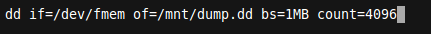
\includegraphics[width=0.9\textwidth]{img/dd.png}
    \end{block}
    
\end{frame}

\begin{frame}
    \frametitle{Analyse du dump}
    \begin{block}{Où trouver la clé de chiffrement ?}
    Clé présente dans le driver de Truecrypt.
    Où trouver le driver ?
    Séparation de la mémoire en 2 espaces
    \begin{itemize}
        \item Mémoire utilisateur
        \item Mémoire noyau 
        \begin{itemize}
        \item Les pool de mémoire non paginée
        \end{itemize}
    \end{itemize}

    \end{block}
    
    Dans certains cas on peut aussi récupérer le mot de passe.
\end{frame}




%%%%%%%%%%%%%%%%%%%%%%%%%%%Conclusion
\section{Conclusion}
\begin{frame}
    Aucune technique n'est infaillible, mais des précautions peuvent être prises:
    \begin{itemize}
        \item Protéger le BIOS par un mot de passe % Vraiment insister sur
        % le fait que ça apporte une protection faible : sautage de pile,
        % extraction de disque, flash de bios facile sur beacoup de laptop
        \item Surveillance de l'appareil
        \item Prendre garde à la veille prolongée
        \item TPM
    \end{itemize}

    \vspace{1cm}
    Chiffrer le disque dur n'est pas une solution miracle, mais protège
    les données en cas de vol non ciblé.
\end{frame}

\begin{frame}
\begin{center}
    {\Huge \alert{Merci de votre attention.}}
    
    {\Huge Avez-vous des questions ?}

    
\includegraphics[height=0.60\textheight]{img/question.jpg}
\end{center}
\end{frame}

\end{document}
